\label{chap:pt1_chapter7}

In Section~\ref{sec:pso_algorithm}, we stated that the linear constraints of the MIP model were used as a reference to model the constraints in PSO and incorporated into its implementation to evaluate the feasibility of the layouts. 

Implementing this approach, however, requires the MIP constraints to be reformulated into a form that can be evaluated by PSO. Since the MIP model was developed in MiniZinc, this reformulation can be avoided by exploiting the FlatZinc file generated during model compilation. The constraint evaluation performed by PSO can then be based directly on the information contained in this file.

This chapter presents the implementation of this solution through the development of a FlatZinc-based PSO algorithm designed to solve MiniZinc models involving continuous variables and nonlinear constraints. Before describing the algorithm in detail, the following sections discuss the structure of the FlatZinc model and how it is represented within the FlatZinc-based PSO.


\section{FlatZinc model and flattening process}
\label{sec:flattening}

The process of converting a MiniZinc model into a FlatZinc model is known as \emph{flattening}. During this process, the variables of the original model are retained, arrays of variables are expanded into indexed variables, and constraints are rewritten into a primitive form supported by the target solver. Listing~\ref{lst:json_example} illustrates this process by presenting the FlatZinc model generated from the MiniZinc model presented in Listing~\ref{lst:minizinc_example}.

\begin{lstlisting}[language=MiniZinc, caption={Example of MiniZinc model}, label={lst:minizinc_example}]
	var -1.0..1.0: x1;
	var -1.0..1.0: x2;
	
	var float: objective =
	pow(x1, 2.0) + pow(x2 - 1.0, 2.0);
	
	constraint x2 - pow(x1, 2.0) = 0.0;
	
	solve minimize objective;
\end{lstlisting}

\begin{lstlisting}[language=json, caption={JSON representation of the FlatZinc model}, label={lst:json_example}]
	{
		"variables": {
			"x1" : { "type" : "float", "domain" : [[-1.0, 1.0]] },
			"x2" : { "type" : "float", "domain" : [[-1.0, 1.0]], "defined" : true },
			"objective" : { "type" : "float", "defined" : true },
			"X_INTRODUCED_1_" : { "type" : "float", "domain" : [[-2.0, 0.0]], "introduced": true, "defined" : true },
			"X_INTRODUCED_2_" : { "type" : "float", "introduced": true, "defined" : true }
		},
		"arrays": {
		},
		"constraints": [
		{ "id" : "float_pow", "args" : ["X_INTRODUCED_1_", 2.0, "X_INTRODUCED_2_"], "defines" : "X_INTRODUCED_2_"},
		{ "id" : "float_pow", "args" : ["x1", 2.0, "x2"], "defines" : "x2"},
		{ "id" : "float_lin_eq", "args" : [[1.0, 1.0, -1.0], ["x2", "X_INTRODUCED_2_", "objective"], -0.0], "defines" : "objective"},
		{ "id" : "float_lin_eq", "args" : [[1.0, -1.0], ["x2", "X_INTRODUCED_1_"], 1.0], "defines" : "X_INTRODUCED_1_"}
		],
		"output": ["x1", "x2"],
		"solve": { "method" : "minimize", "objective" : "objective" },
		"version": "1.0"
	}
\end{lstlisting}


The flattening process may introduce new variables, whose values may or may not be defined by existing constraints. For instance, for the model in Listing~\ref{lst:minizinc_example}, the flattening process introduces two new variables, \texttt{X\_INTRODUCED\_1\_} and \texttt{X\_INTRODUCED\_2\_}, defined in lines 6--7 of Listing~\ref{lst:json_example}. These variables represent, respectively, a linear transformation of $x2$ and the result of the operation $(x2-1)^2$. 

In the FlatZinc model, constraints that determine the values of variables are identified by the \texttt{defines} attribute, which specifies the corresponding variable. Identifying these variables is important because their values can be computed from the corresponding constraint rather than determined through the search. For instance, in Listing~\ref{lst:json_example}, all constraints define a variable.


\section{Invariant graph}

Once the details contained in the FlatZinc model have been extracted, they must be represented in a form suitable for evaluation by PSO. In Constraint-Based Local Search (CBLS), models are typically represented as directed graphs linking variables to the constraints in which they occur. This representation is known as the \emph{invariant graph}~\cite{lewander2025invariant}.

In the invariant graph, defined variables have a single incoming edge corresponding to the constraint that assigns their value, as well as outgoing edges to the constraints in which they are involved. Decision variables, in contrast, have no incoming edges and only outgoing edges associated with the constraints in which they participate.

Figure~\ref{fig:invariant_graph} represents the invariant graph of the MiniZinc model presented in Listing~\ref{lst:minizinc_example}, although the model specifies two variables, $x1$ and $x2$, the flattening process identifies only $x1$ as a decision variable. The variable $x2$ is defined by the \texttt{float\_pow} constraint, which assigns its value and is therefore connected to $x2$ through an incoming edge.

The invariant graph allows the values of defined variables to be computed by traversing the graph according to a topological ordering of the constraints. Consequently, when PSO is used to search for a solution, it only needs to assign values to the decision variables that are not defined.

\begin{figure}[t]
	\centering
	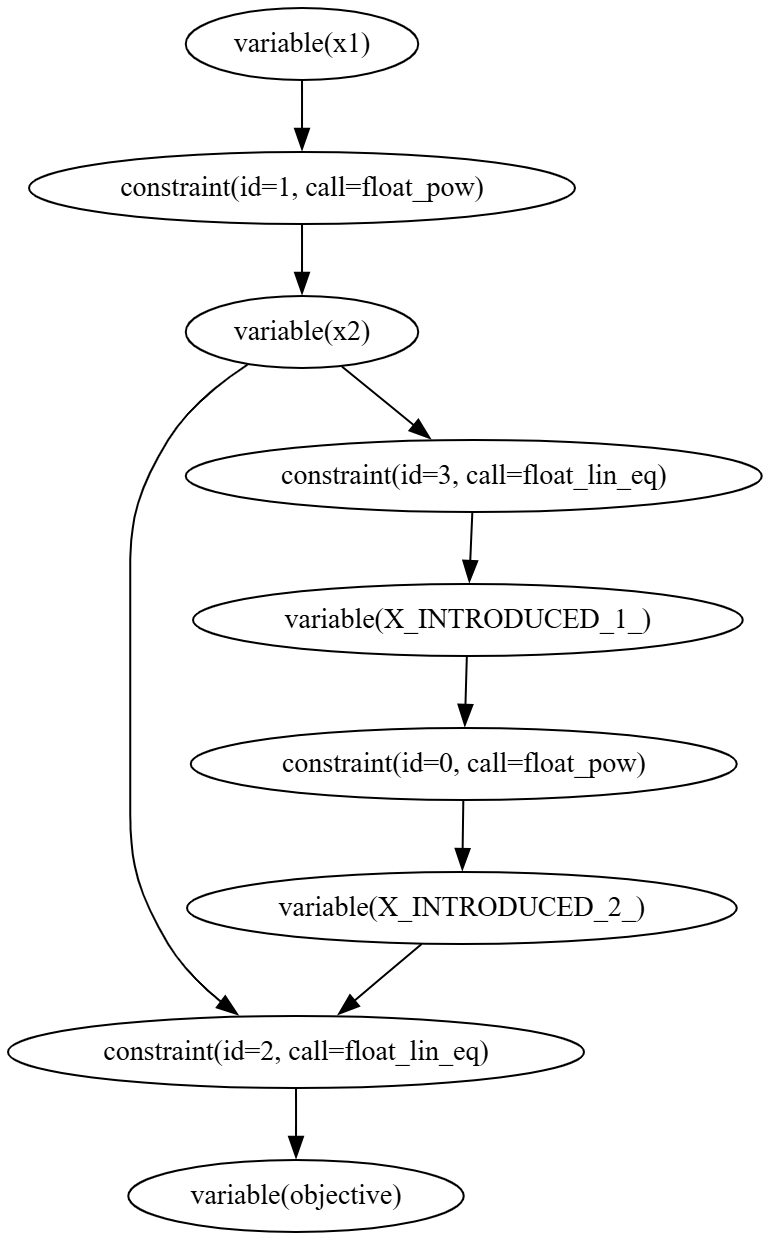
\includegraphics[width=0.4\linewidth]{figures/invariant_graph.png}
	\caption{Example of invariant graph}
	\label{fig:invariant_graph}
\end{figure}

\section{Integrating FlatZinc and PSO}
\label{sec:fzn_integration_pso}

Solving a constraint optimization problem with PSO using the information contained in the FlatZinc model and soft constraints requires associating each built-in FlatZinc function with a corresponding violation function.

In Flatzinc-based PSO, each violation function measures the distance from the feasible region, as this strategy has been shown to be more effective than death-based penalties~\cite{pulido2004constraint, mezura2011constraint}. For instance, the constraint \texttt{float\_pow} is represented in FlatZinc by the built-in function:

\[ \texttt{float\_pow}(\texttt{var float:} x,\texttt{var float:} y, \texttt{var float:} z)\]

\noindent corresponding to the relation $z = x^y$. Its violation can therefore be expressed as:

\[\max\left(|x^y - z|, 0\right)\].

The FlatZinc-based PSO must assign a value to each decision variable identified in the invariant graph $\mathcal{G}$ derived from the MiniZinc model. Therefore, the position of each particle $s \in [1..\swarmsize]$ is represented by an array $p_s$ of dimension $d$, where $d$ is the number of decision variables in $\mathcal{G}$.

Once the particle position $p_s$ has been determined, the values of the defined variables are computed by traversing the constraints in $\mathcal{G}$ according to their topological order, and the violation of each constraint is evaluated using its corresponding violation function.

The overall constraint violation associated with particle $p_s$ is computed as the sum of the violations of all constraints represented in $\mathcal{G}$:

\[
cv(p_s)=\sum_{c\in\mathcal{C}}cv_c(p_s),
\]

\noindent where $\mathcal{C}$ denotes the set of constraints represented in the invariant graph $\mathcal{G}$, and $cv_c(p_s)$ denotes the violation associated with constraint $c$.

\begin{algorithm}[htbp]
	\footnotesize
	\caption{FlatZinc-Based Particle Swarm Optimization initialization phase}
	\label{alg:fzn_pso_pt1}
	\begin{algorithmic}[1]
		\Require Swarm size $\swarmsize$, maximum number of iterations $\maxiter$, inertia weight $w$, cognitive coefficient $c_1$, social coefficient $c_2$, invariant graph $\mathcal{G}$
		\Ensure Best solution found $p^*$
		
		\State Let $d$ be the number of variables identified in $\mathcal{G}$
		\label{alg:start_init}
		
		\For{$s=1$ to $\swarmsize$}
		\State Randomly initialize $p_s$ within the bounds of the variables in $\mathcal{G}$
		\State Randomly initialize velocity vector $v_s$
		\State $k_s\gets0$
		\label{alg:end_init}
		
		\State Evaluate $p_s^*$ computing $cv(p_s^*)$ and $f(p_s^*)$
		\label{alg:init_eval}
		\State $p_s^* \gets p_s$
		\label{alg:start_init_update}
		\If{$cv(p_s^*)=0$}
		\If{$f(p_s^*) < f(p^*)$}
		\State $p^*\gets p_s^*$
		\EndIf
		\ElsIf{$cv(p_s^*) < cv(p^*)$}
		\State $p^*\gets p_s^*$
		\EndIf
		\label{alg:end_init_update}
		
		\EndFor
		\algstore{part1}
	\end{algorithmic}
\end{algorithm}

\begin{algorithm}
	\caption{FlatZinc-Based Particle Swarm Optimization search phase}
	\label{alg:fzn_pso_pt2}
	\begin{algorithmic}[1]
		\algrestore{part1}
		\For{$k=1$ to $\maxiter$}
		\For{$s=1$ to $\swarmsize$}
		
		\For{$i=1$ to $d$}
		\State Randomly generate $r_1,r_2\in[0,1]$
		\label{alg:start_update}
		\State $v_s[i]\gets wv_s[i]+c_1r_1(p_s^*[i]-p_s[i])+c_2r_2(p^*[i]-p_s[i])$
		\label{alg:end_update}
		
		
		\State Randomly generate $\rho\in[0,1]$
		\label{alg:start_noise}
		\If{$\rho<0.5$}
		\State Randomly generate $\epsilon\in[-\delta,\delta]$
		\State $v_s[i]\gets v_s[i]+\epsilon$
		\Comment{Perturbed velocity}
		\EndIf
		\label{alg:end_noise}
		
		\State $p_s[i]\gets p_s[i]+v_s[i]$
		\label{alg:start_second_eval}
		\EndFor
		
		\State Evaluate $p_s$ and compute $cv(p_s)$ and $f(p_s)$
		\label{alg:end_second_eval}
		
		\If{$k_s=k_{\max}$}
		\label{alg:start_stagnation}
		\Comment{Stagnation prevention}
		\State Reinitialize $p_s$ and $v_s$
		\State $p_s^*\gets p_s$
		\State $k_s\gets0$
		\EndIf
		\label{alg:end_stagnation}
		
		\If{$cv(p_s)=0$ \textbf{and} $cv(p_s^*)=0$}
		\label{alg:start_deb}
		\If{$f(p_s) < f(p_s^*)$}
		\State $p_s^*\gets p_s$
		\State $k_s\gets0$
		\If{$f(p_s*) < f(p^*)$}
		\State $p^*\gets p_s^*$
		\EndIf
		\EndIf
		\ElsIf{$cv(p_s) < cv(p_s^*)$}
		\State $p_s^*\gets p_s$
		\State $k_s\gets0$
		\Else
		\State $k_s\gets k_s+1$
		\EndIf
		\label{alg:end_deb}
		
		\EndFor
		
		\EndFor
		
		\State \Return $p^*$
		
	\end{algorithmic}
\end{algorithm}

Algorithms~\ref{alg:fzn_pso_pt1} and~\ref{alg:fzn_pso_pt2} present the pseudocode of the FlatZinc-based PSO. The algorithm takes as input the swarm size $\swarmsize$, the maximum number of iterations $\maxiter$, the inertia weight $w$, the cognitive coefficient $c1$, the social coefficient $c2$, and the invariant graph $\mathcal{G}$ of the FlatZinc model. It returns the best solution found by the swarm, denoted by $p^*$.

At the beginning of the initialization phase in lines~\ref{alg:start_init}--\ref{alg:end_init} of Algorithm~\ref{alg:fzn_pso_pt1}, each particle is initialized from the invariant graph $\mathcal{G}$ by considering the number of decision variables $d$ and their corresponding bounds. The particle position $p_s$ and velocity $v_s$ are randomly initialized, and a stagnation counter $k_s$ is set to zero. The counter tracks the number of consecutive iterations in which the particle fails to improve its personal best. Since strict adherence to Deb's rules can lead to premature convergence, the particle is reinitialized when the counter reaches a predefined threshold, promoting exploration and helping the search escape local optima.

Once the first position is assigned, each particle is evaluated in terms of objective value and constraint violations, as described in line~\ref{alg:init_eval} of Algorithm~\ref{alg:fzn_pso_pt1}. In this phase, the solution proposed by the particle is injected into the invariant graph $\mathcal{G}$ and the values of the defined variables as well as the constraint violations are computed.

At the end of the evaluation (lines~\ref{alg:start_init_update}--\ref{alg:end_init_update} of Algorithm~\ref{alg:fzn_pso_pt1}), the personal best position $p_s^*$ of each particle is set to its first evaluated solution, and the global best solution $p^*$ is updated considering the best candidate found among all particles.

During the search phase, in lines~\ref{alg:start_update}--\ref{alg:end_update} of Algorithm~\ref{alg:fzn_pso_pt2}, the velocity of each particle is iteratively update according to the standard PSO equations. 

In lines~\ref{alg:start_noise}--\ref{alg:end_noise} of Algorithm~\ref{alg:fzn_pso_pt2}, uniformly sampled noise $\epsilon \in (-\delta,\delta)$ is added to the particle velocity when a randomly generated value $\rho$ is below $0.5$. These perturbations allow particles to occasionally deviate from their current trajectories, helping them escape local optima and promoting broader exploration of the search space~\cite{hu2002solving}.

After updating the velocity, the position is updated accordingly, and the particle is evaluated in terms of constraint violation and objective function (lines~\ref{alg:start_second_eval}--\ref{alg:end_second_eval} of Algorithm~\ref{alg:fzn_pso_pt2}).

At the end of the evaluation, the stagnation mechanism is applied. If a particle does not improve its personal best for $k_{\max}$ consecutive iterations, it is reinitialized as described in lines~\ref{alg:start_stagnation}--\ref{alg:end_stagnation} of Algorithm~\ref{alg:fzn_pso_pt2}.

Candidate solutions are compared using Deb's rules, and after updating the personal best positions, the global best solution $p^*$ is updated accordingly as illustrated in lines~\ref{alg:start_deb}--\ref{alg:end_deb}  of Algorithm~\ref{alg:fzn_pso_pt2}. Finally, at the end of the optimization process, the best solution found is returned.


\section{Evaluation}
To evaluate the effectiveness of the proposed integration, the algorithm described in Section~\ref{sec:fzn_integration_pso} was compared with a non-FlatZinc PSO implementation. Both algorithms adopt the same search strategy; the only difference is that the FlatZinc-based PSO derives the variables and constraints from the FlatZinc model, whereas the non-FlatZinc implementation directly encodes the problem variables and constraints in the PSO code.

The two approaches were evaluated on the benchmark problems presented in~\cite{hu2002solving} and~\cite{parsopoulos2002particle}, comprising a total of 15 problems\footnote{Problems 3 and 4 presented in~\cite{parsopoulos2002particle} correspond to problems g09 and g04 presented in~\cite{hu2002solving}, respectively, whereas problem 5 represents a variant of problem 4 for which the solution is unknown.}.The experiments were conducted on a 64-bit Windows machine equipped with an Intel Core i5 processor and 16~GB of RAM. 

To ensure a fair comparison between the two approaches, the hyperparameters were set to those presented in Section~\ref{sec:evaluation}, which were shown to be effective in guiding the PSO search towards high-quality solutions for constraint optimization problems. Since the benchmark problems are less complex and involve fewer constraints than those considered for fixture layout optimization, only the \texttt{swarm\_size} and \texttt{max\_iteration} parameters were reduced, to 100 and 500, respectively.

\begin{table}[t]
	\centering
	\footnotesize
	\caption{Comparison between FlatZinc-based PSO and non-FlatZinc PSO. The best value (closest to the optimum) is highlighted in bold when there is a difference between the values proposed.}
	\label{tab:fzn_pso_comparison}
	\setlength{\tabcolsep}{5pt}
	\begin{tabular}{cccccc}
		\toprule
		\textbf{Problem} & \textbf{Optimum} & \textbf{Best fzn-PSO} & \textbf{Best PSO} & \textbf{Mean fzn-PSO} & \textbf{Mean PSO} \\
		\midrule
		g01 & -15.000 & \textbf{-14.892} & -14.825 & \textbf{-13.025} & -12.887 \\
		\midrule
		g02 & -0.804 & \textbf{-0.345} & -0.341 & -0.281 & \textbf{-0.298} \\
		\midrule
		g03 & -1.000 & \textbf{-0.956} & -0.947 & \textbf{-0.895} & -0.785 \\
		\midrule
		g04 & -30665.386 & \textbf{-30666.331} & -30666.226 & \textbf{-30665.388} & -30664.476 \\
		\midrule
		g05 & 5126.496 & -- & -- & -- & -- \\
		\midrule
		g06 & -6961.813 & -6951.099 & \textbf{-6953.812} & \textbf{-6922.202} & -6904.423 \\
		\midrule
		g07 & 24.306 & \textbf{32.896} & 33.607 & 71.290 & \textbf{47.094} \\
		\midrule
		g08 & 0.095 & -0.096 & -0.096 & -0.096 & -0.096 \\
		\midrule
		g09 & 680.630 & \textbf{684.614} & 685.152 & \textbf{687.721} & 689.371 \\
		\midrule
		g10 & 7049.248 & \textbf{8015.163} & 8283.200 & 12657.795 & \textbf{10026.341} \\
		\midrule
		g11 & 0.750 & \textbf{0.750} & 0.749 & \textbf{0.750} & 0.749 \\
		\midrule
		g12 & -1.000 & -1.000 & -1.000 & -1.000 & -1.000 \\
		\midrule
		problem 1 & 1.393 & 1.999 & \textbf{1.392} & 1.999 & \textbf{1.392} \\
		\midrule
		problem 2 & -6961.813 & -6946.519 & \textbf{-6953.812} & \textbf{-6922.013} & -6904.063 \\
		\midrule
		problem 6 & -213.000 & -211.501 & -211.501 & -211.501 & -211.501 \\
		\bottomrule
	\end{tabular}
\end{table}

Table~\ref{tab:fzn_pso_comparison} presents the results of the comparison between the FlatZinc-based PSO and the non-FlatZinc PSO. The results are evaluated on 50 independent runs for each problem, using the same random seed for both algorithms to ensure identical initial conditions. Results for problem g05 are omitted, as neither algorithm was able to find a feasible solution.

Considering the results reported in the table for the mean, the FlatZinc-based PSO achieves better performance in 7 of the 15 problems, while the two approaches obtain identical results in 3 problems. Among the remaining cases, excluding g05, the non-FlatZinc PSO performs better in 4 problems.

Since both algorithms share the same search mechanism, the observed performance differences can primarily be attributed to the information provided by the FlatZinc model. As described in Section~\ref{sec:flattening}, the flattening process produces a more explicit representation of the original model, decomposing complex constraints and identifying defined variables. This additional information allows constraint violations to be evaluated in greater detail and can reduces the number of variables that must be directly searched.

\begin{table}[t]
	\centering
	\footnotesize
	\caption{Runtime comparison between FlatZinc-PSO and non-FlatZinc PSO.}
	\label{tab:runtime_comparison}
	\setlength{\tabcolsep}{5pt}
	\begin{tabular}{ccc}
		\toprule
		\textbf{Problem} & \textbf{fzn-PSO (ms)} & \textbf{PSO (ms)} \\
		\midrule
		
		g01 & 2260.000 & 1500.000 \\
		\midrule
		
		g02 & 6930.000 & 2510.000 \\
		\midrule
		
		g03 & 2130.000 & 1210.000 \\
		\midrule
		
		g04 & 1660.000 & 626.760 \\
		\midrule
		
		g05 & -- & -- \\
		\midrule
		
		g06 & 984.960 & 265.970 \\
		\midrule
		
		g07 & 3040.000 & 1220.000 \\
		\midrule
		
		g08 & 878.160 & 266.950 \\
		\midrule
		
		g09 & 1900.000 & 864.160 \\
		\midrule
		
		g10 & 1670.000 & 934.520 \\
		\midrule
		
		g11 & 419.950 & 266.350 \\
		\midrule
		
		g12 & 1550.000 & 726.060 \\
		\midrule
		
		problem 1 & 702.450 & 153.410 \\
		\midrule
		
		problem 2 & 874.010 & 265.710 \\
		\midrule
		
		problem 6 & 1210.000 & 698.410 \\
		
		\bottomrule
	\end{tabular}
\end{table}


However, the processing of this additional information comes at the cost of more computational overhead. Table~\ref{tab:runtime_comparison} reports the runtimes, in milliseconds, required by the FlatZinc-based PSO and the non-FlatZinc PSO to complete 500 iterations. On average, the non-FlatZinc PSO is approximately 2.55 times faster than the FlatZinc-based PSO.

To assess whether the observed differences in solution quality are statistically significant, a \emph{Wilcoxon signed-rank test}~\cite{woolson2007wilcoxon} was performed on the results of the 50 runs for each benchmark problem. This test compares two related samples by ranking the absolute differences between paired observations and assessing whether these differences are systematically positive or negative. The resulting $p_{value}$ measures the evidence against the null hypothesis that the two methods produce equivalent results; a value of $p_{value}<0.05$ is considered to indicate a statistically significant difference between the two methods. 

\begin{table}[t]
	\centering
	\footnotesize
	\caption{Wilcoxon signed-rank test p-values comparing FlatZinc PSO and non-Flatzinc PSO across benchmark problems. Values with $p_{value} < 0.05$ are highlighted in bold.}
	\label{tab:wilcoxon_pvalues}
	\setlength{\tabcolsep}{5pt}
	\begin{tabular}{cc}
		\toprule
		\textbf{Problem} & \textbf{Wilcoxon $p_{value}$} \\
		\midrule
		
		g01 & 0.1781 \\
		\midrule
		
		g02 & \textbf{0.001191} \\
		\midrule
		
		g03 & \textbf{2.994e-11} \\
		\midrule
		
		g04 & \textbf{1.867e-07} \\
		\midrule
		
		g05 & -- \\
		\midrule
		
		g06 & \textbf{0.003205} \\
		\midrule
		
		g07 & 0.2115 \\
		\midrule
		
		g08 & \textbf{6.825e-05} \\
		\midrule
		
		g09 & \textbf{0.007844} \\
		\midrule
		
		g10 & \textbf{0.0009504} \\
		\midrule
		
		g11 & \textbf{1.776e-15} \\
		\midrule
		
		g12 & \textbf{8.882e-15} \\
		\midrule
		
		problem 1 & \textbf{1.776e-15} \\
		\midrule
		
		problem 2 & \textbf{0.01026} \\
		\midrule
		
		problem 6 & \textbf{0.005942} \\
		
		\bottomrule
	\end{tabular}
\end{table}

Table~\ref{tab:wilcoxon_pvalues} reports the corresponding $p_{value}$ obtained from the run-by-run comparison of the FlatZinc-based PSO and the non-FlatZinc PSO for the benchmark problems. Overall, statistically significant differences were found for 12 of the 15 benchmark problems considered, indicating that the two approaches produce significantly different solution qualities in the majority of the cases.


